\subsection{\textit{Front-end}}
\subsubsection{\textit{Root} della \textit{repository} e \textit{file} di configurazione}

\begin{figure}[H]
      \centering
      %\hspace{-3.25cm} % Sposta la figura a sinistra di n cm
      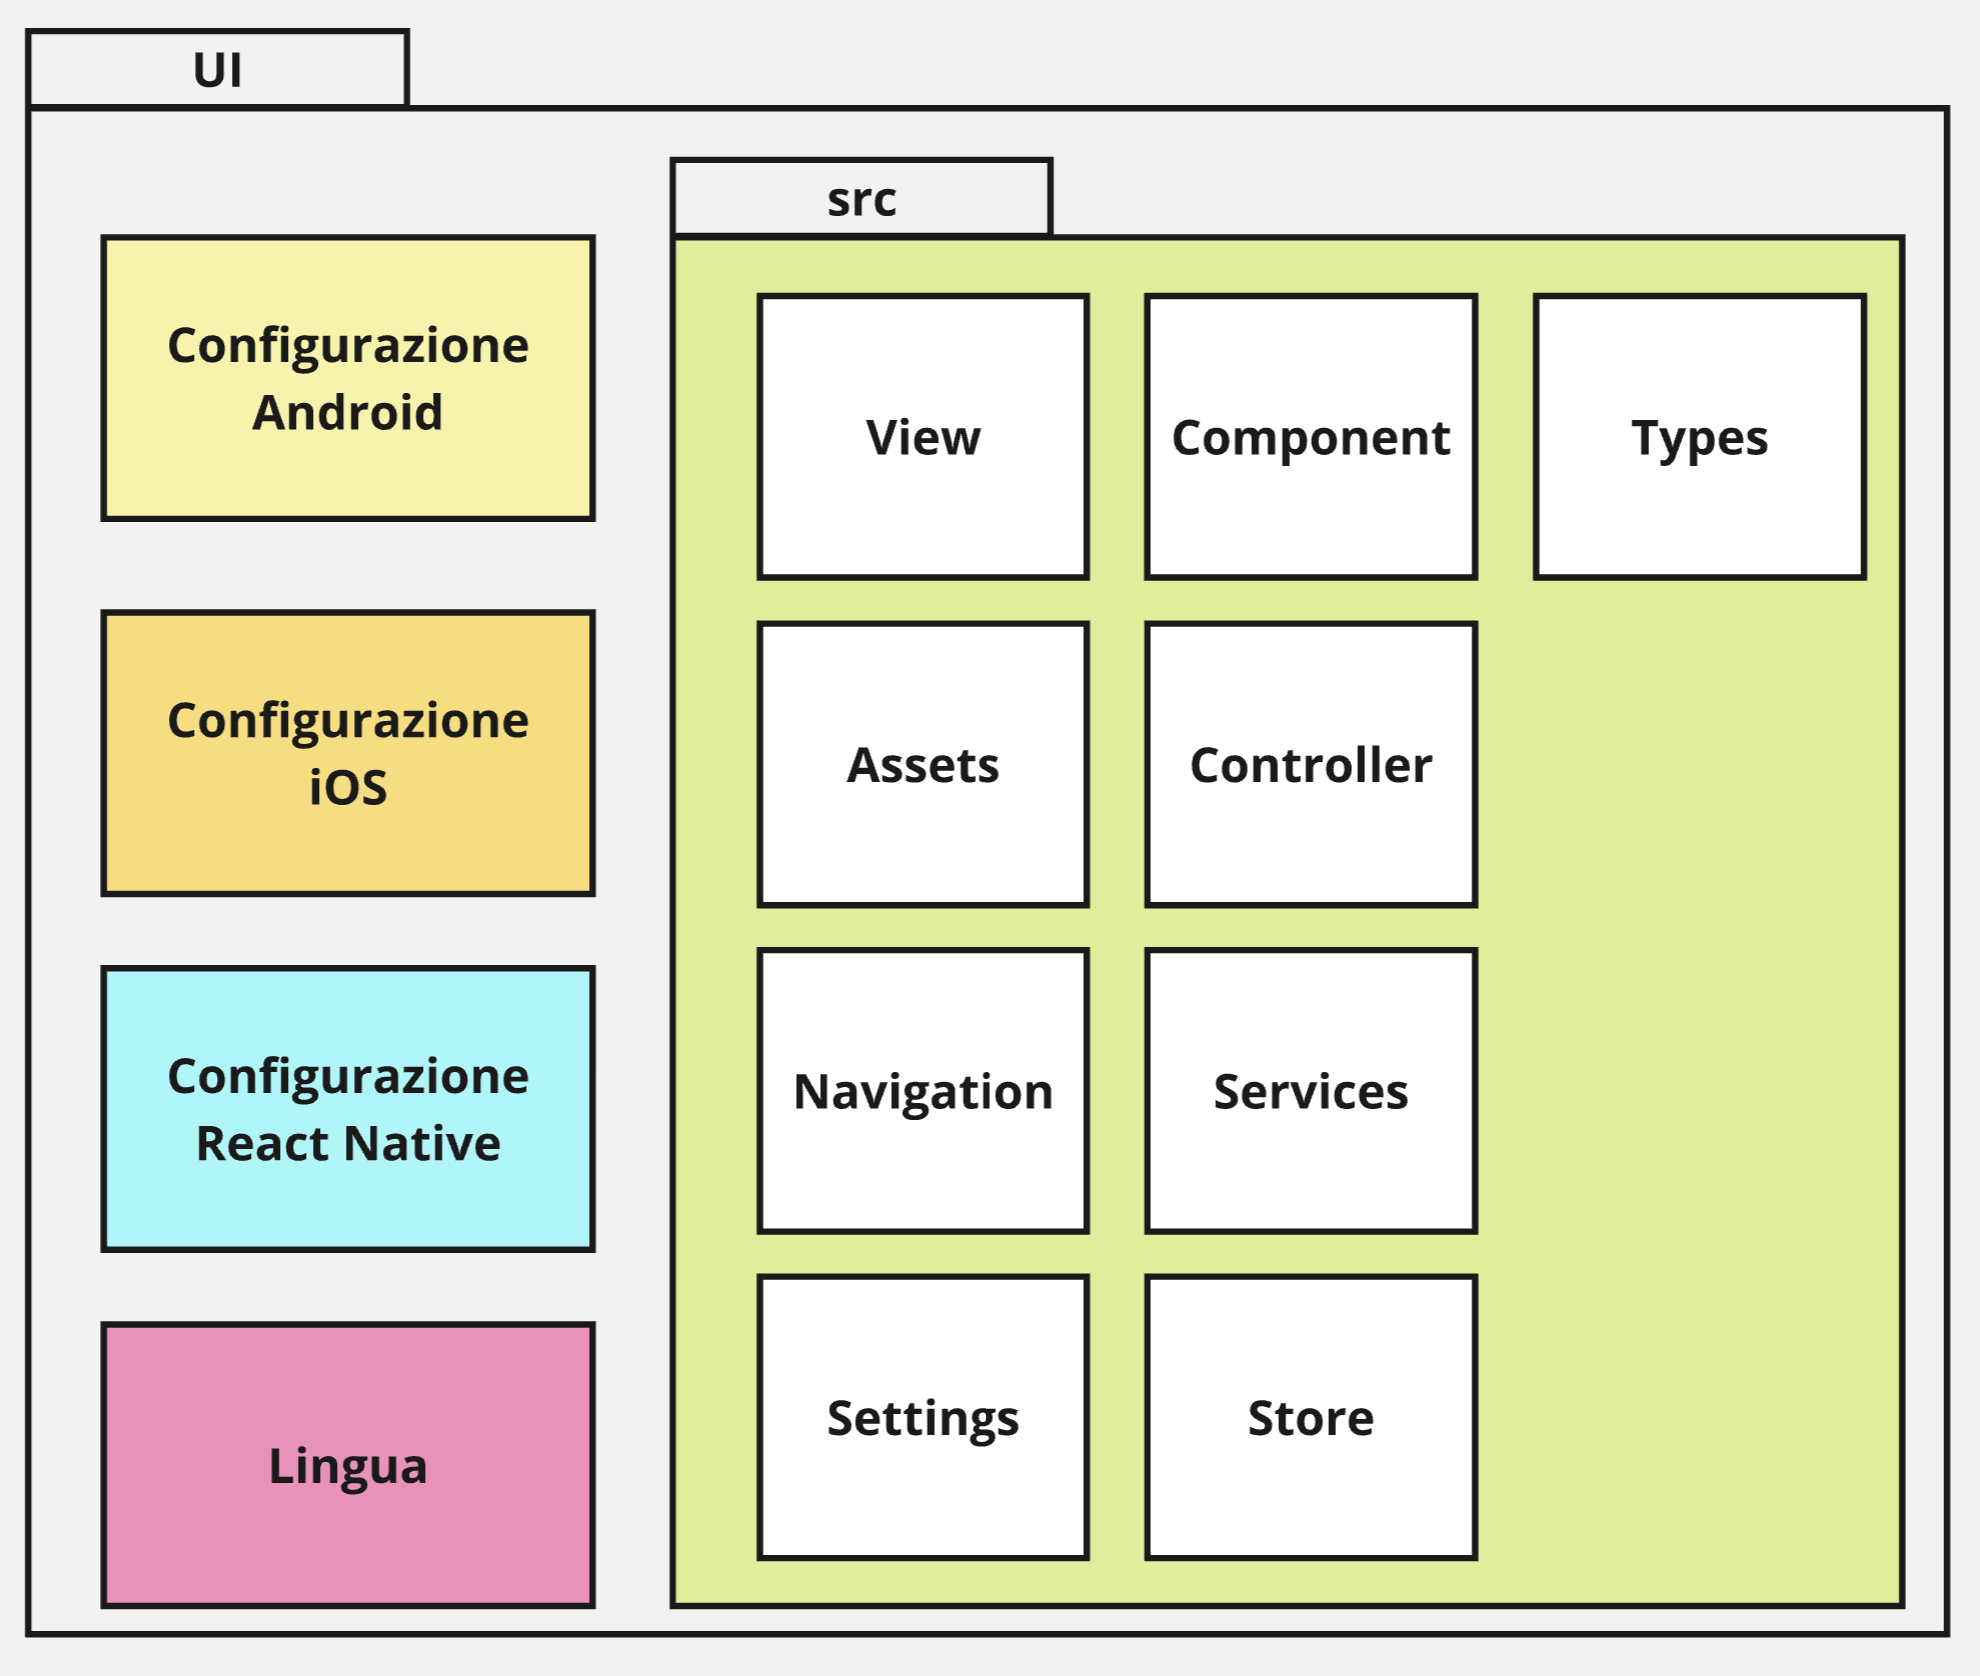
\includegraphics[width=0.6\textwidth]{img/architettura_ui.png}
      \caption{\textit{Root} della \textit{repository} che contiene il \textit{front-end}}
      \label{fig:ui architecture}
\end{figure}

Prima di descrivere l'architettura del \textit{front-end} soffermiamoci ad analizzare il contenuto del \textit{root} della \textit{repository} 
mostrata dalla figura \ref{fig:ui architecture}.
Qui sono contenuti i file di configurazione di React Native e le impostazioni dei compilatori.\\
La \textit{repository} è suddivisa nelle seguenti cartelle:
\begin{itemize}
    \item \texttt{\textbf{Android}}: specifica per React Native, contiene i file di configurazione 
          per la versione Android dell'\textit{app} e \textit{file} come \texttt{build.gradle} e \texttt{AndroidManifest.xml} 
          per la configurazione del compilatore Android;
    \item \texttt{\textbf{iOS}}: specifica per React Native, contiene il progetto Xcode e i file di configurazione 
          per la versione iOS dell'\textit{app} e \textit{file} per la configurazione del compilatore di iOS;
    \item \texttt{\textbf{lang}}: contiene i \textit{file} \texttt{en.json e it.json} che definiscono il testo usato nell'
          applicazione nelle lingue italiano e inglese;
    \item \texttt{\textbf{src}}: contiene tutto il codice del \textit{front-end} e realizza l'architettura;
    \item \textbf{Altri \textit{file} di configurazione}: questi \textit{file} sono fondamentali 
          per garantire un corretto funzionamento e una gestione efficiente del progetto, qui riporto quelli più importanti:
          \begin{itemize}
            \item \textbf{\texttt{package.json}}: contiene le informazioni sul progetto come il nome del progetto, versione,
                  \textit{script} di comando e dipendenze. È il \textit{file} principale per gestire i pacchetti Node.js utilizzati nel progetto;
            \item \textbf{\texttt{yarn.lock}}: questo \textit{file} viene generato automaticamente quando si genera il progetto e 
                  permette di gestire ed installare le dipendenze con le loro versioni esatte;
            \item \textbf{\texttt{metro.config.js}}: configura Metro, il \textit{bundler} di JavaScript predefinito 
                  per React Native. Un \textit{bundler} è uno strumento di sviluppo \textit{software} che combina diversi 
                  \textit{file} di codice sorgente e le loro dipendenze in uno o più \textit{file} ottimizzati, pronti per essere distribuiti 
                  o eseguiti in un ambiente di produzione. Questo \textit{file} permette di personalizzare il comportamento di Metro, come 
                  l'aggiunta di \textit{alias, path} personalizzati, o l'esclusione di determinati \textit{file} dalla \textit{build}.
            \item \textbf{\texttt{babel.config.js}}: configura Babel, il \textit{transpiler} di JavaScript. 
                  Definisce come il codice deve essere trasformato per essere compatibile con le varie versioni di JavaScript e i 
                  diversi ambienti in cui verrà eseguito.
            \item \textbf{\texttt{index.js}}: punto d'ingresso principale dell'applicazione React Native. Qui viene 
                  avviato il \textit{rendering} del componente radice dell'\textit{app};
            \item \textbf{\texttt{app.tsx}}: contiene il componente radice dell'applicazione. Qui vengono definiti l'interfaccia 
                  utente principale e la logica di base dell'\textit{app}.
            \item \textbf{\texttt{tsconfig.json}}: configura il compilatore TypeScript, specificando le opzioni di compilazione 
            e il comportamento del \textit{transpiling} del codice TypeScript in JavaScript.
          \end{itemize}
\end{itemize}
\subsubsection{Architettura React}

\begin{figure}[H]
      \centering
      %\hspace{-3.25cm} % Sposta la figura a sinistra di n cm
      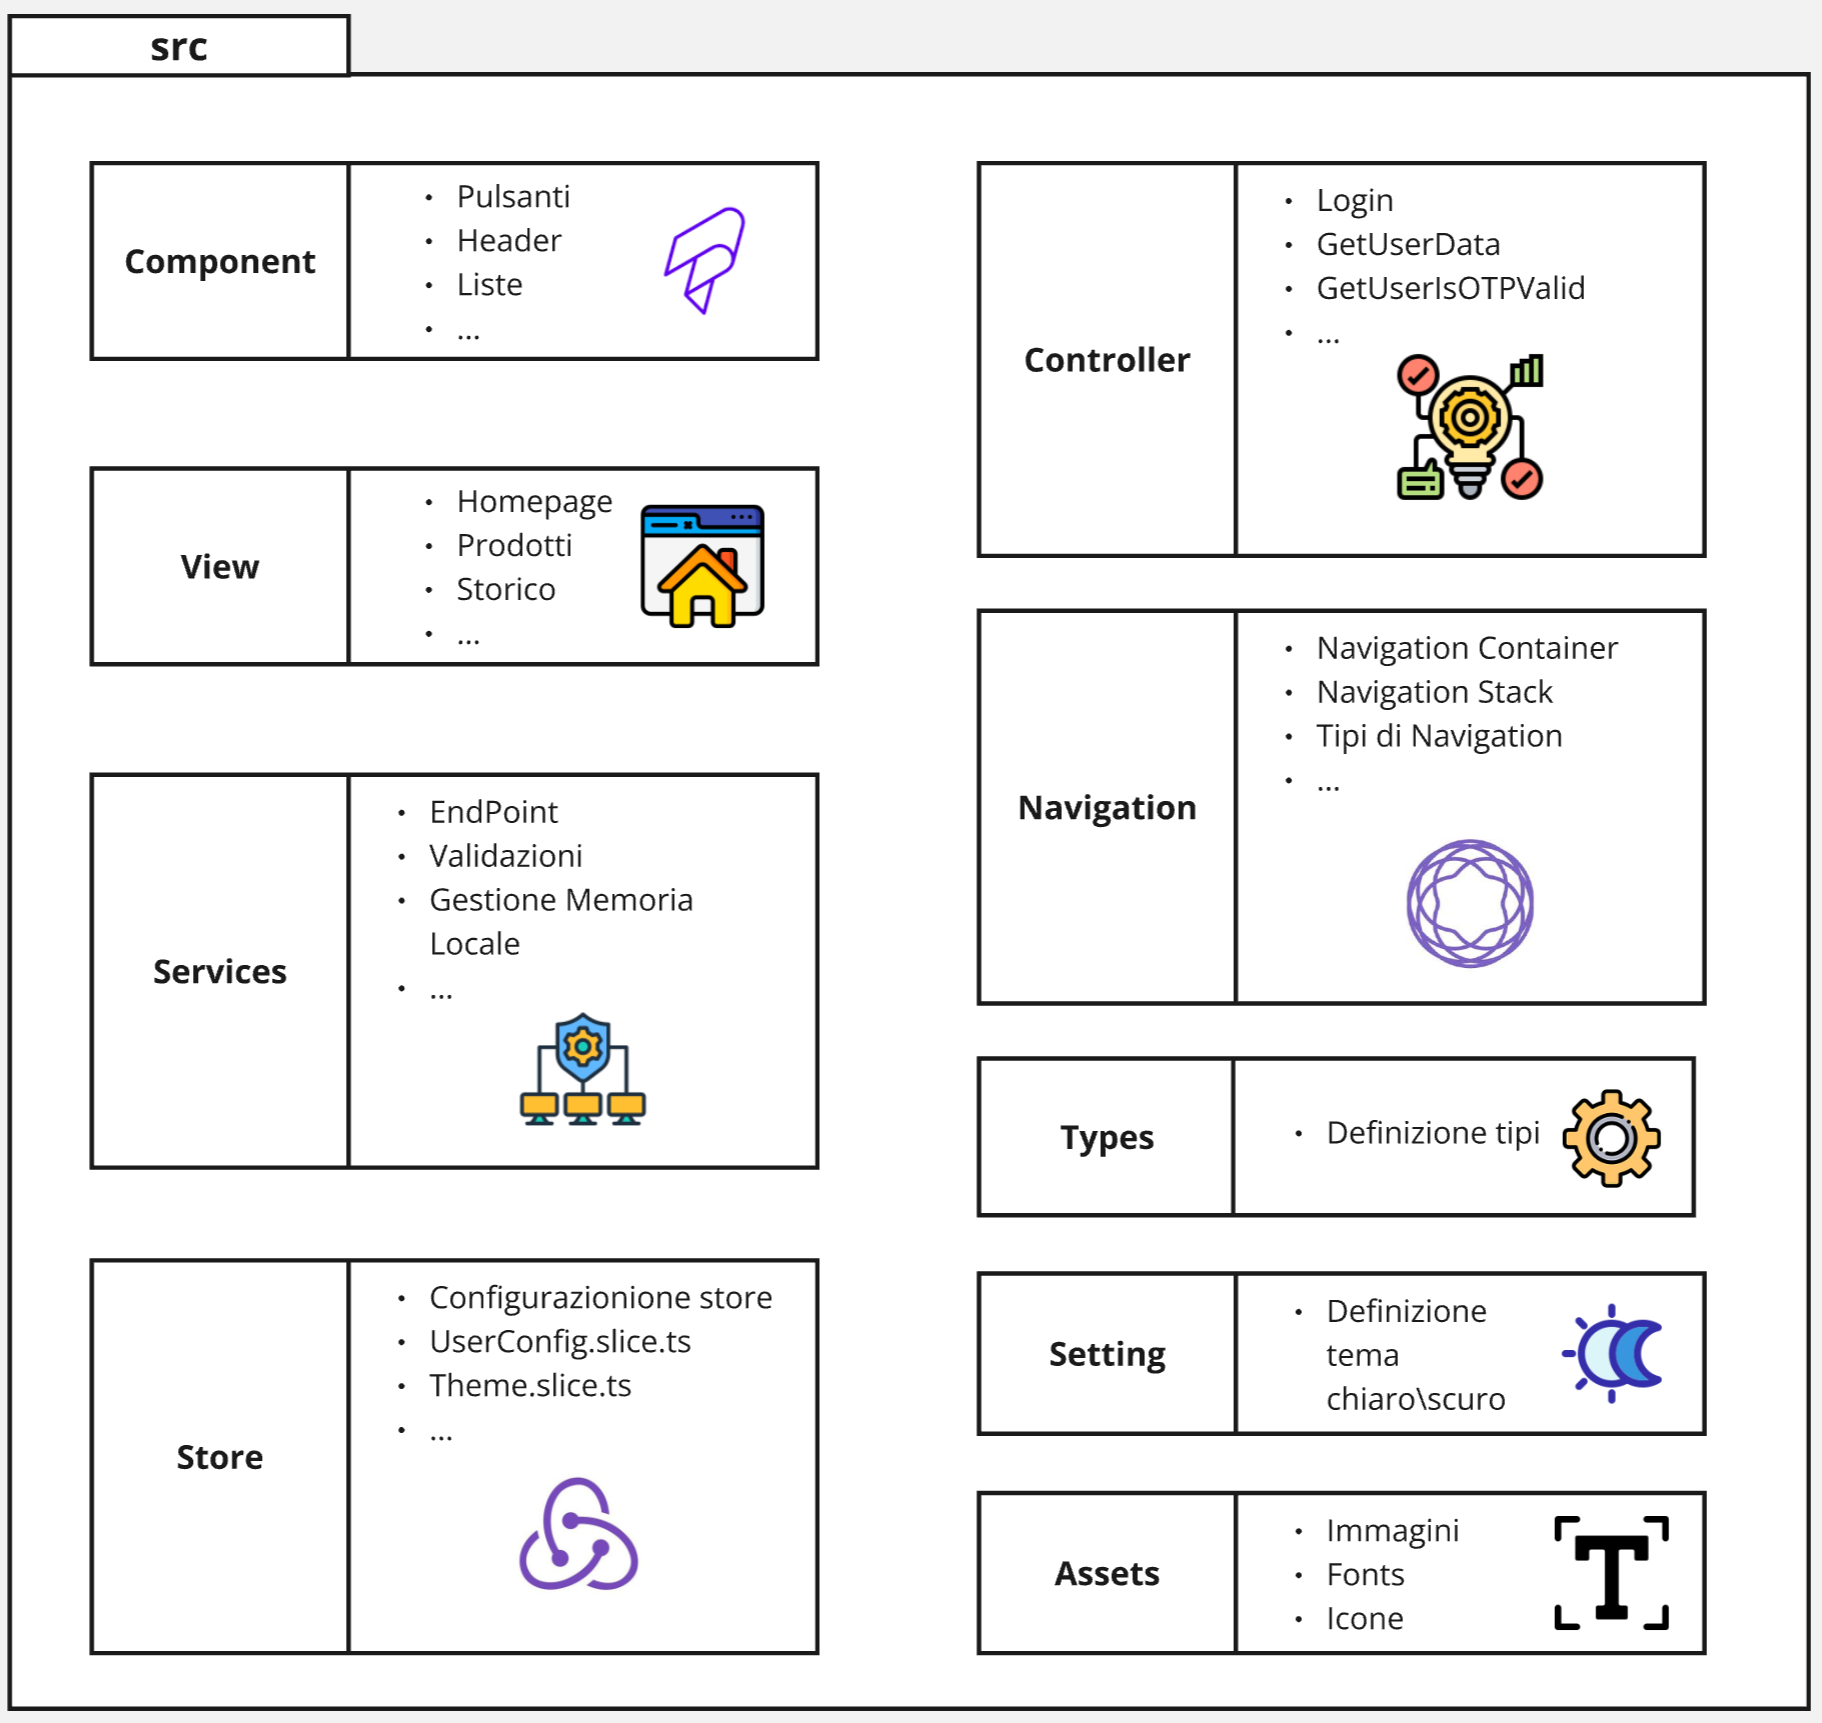
\includegraphics[width=0.8\textwidth]{img/react_architecture.png}
      \caption{Rappresentazione dell'architettura React per {\movi}}
      \label{fig:frontend architecture}
\end{figure}

Una caratteristica distintiva di React è la sua flessibilità nell'implementazione dell'architettura dell'applicazione, 
distinguendosi da altri \textit{framework} JavaScript che impongono modelli predefiniti. Questa libertà consente 
agli sviluppatori di strutturare l'applicazione in base alle specifiche esigenze del progetto.\\
L'architettura React, come illustrata la figura \ref{fig:frontend architecture}, si configura come un insieme di 
componenti responsabili della costruzione dell'interfaccia utente (UI) del \textit{software}. Questa architettura 
può essere concepita come un'organizzazione del codice che facilita la realizzazione di progetti personalizzati, 
includendo vari elementi UI quali pulsanti, moduli, servizi \gls{api} e sistemi di gestione dello stato.\\
L'architettura si articola nelle seguenti directory principali:

\begin{itemize}
      \item \textbf{\texttt{View}}: contiene le pagine complete dell'applicazione, composizioni di 
            componenti più piccoli che formano l'interfaccia utente. Le viste gestiscono la logica e 
            l'organizzazione dei componenti per creare l'esperienza utente complessiva;
      \item \textbf{\texttt{Component}}: ospita componenti UI riutilizzabili e modulari. Questi possono 
            essere elementi come pulsanti, \textit{form}, barre di navigazione o qualsiasi altro elemento 
            dell'interfaccia che può essere utilizzato in più parti dell'applicazione. I componenti in 
            questa cartella sono generalmente più piccoli e più specifici rispetto alle viste;
      \item \textbf{\texttt{Controller}}: contiene la logica di \textit{business} dell'applicazione. Qui 
            si trovano le funzioni e le classi che gestiscono la logica applicativa, elaborano i dati e coordinano le 
            interazioni tra i vari componenti e servizi;
      \item \textbf{\texttt{Services}}: gestisce le interazioni con risorse esterne, come chiamate \gls{api} o la memoria
            del dispositivo. Questa cartella contiene il codice per la comunicazione con il \textit{back-end}, la gestione delle 
            richieste HTTP e l'elaborazione delle risposte. Qui sono definiti inoltre gli \textit{endpoint} per la connessione 
            alle \gls{api};
      \item \textbf{\texttt{Store}}: centralizza la gestione dello stato dell'applicazione utilizzando Redux. Questa cartella 
            contiene la configurazione dello \textit{store} Redux e i \textit{reducer} che definiscono come lo stato dell'applicazione 
            cambia in risposta alle azioni e  dei selettori per accedere allo stato;
      \item \textbf{\texttt{Navigation}}: implementa la logica di \textit{routing} e navigazione dell'applicazione utilizzando 
            React Navigation. Include la mappatura tra i nomi dei \textit{routers} (component che definiscono lo stato della navigazione) 
            e le \textit{view} corrispondenti, nonché opzioni di configurazione per ogni schermata come titoli e animazioni di transizione;
      \item \textbf{\texttt{Types}}: questa cartella contiene le definizioni dei tipi personalizzati utilizzati in tutta l'applicazione. 
            Ciò include interfacce, tipi e enumerazioni che aiutano a mantenere il codice tipizzato e più robusto;
      \item \textbf{\texttt{Assets}}: contiene risorse statiche come immagini, icone, \textit{font} e altri \textit{file} multimediali 
            utilizzati nell'applicazione. Queste risorse sono accessibili e utilizzabili in tutto il progetto;
      \item \textbf{\texttt{Setting}}: definisce i \textit{file} di configurazione per temi (chiaro/scuro).
\end{itemize}